\vspace{-10pt}
\section{Conclusions}
\vspace{-5pt}

\begin{figure}[t]
	\centering
	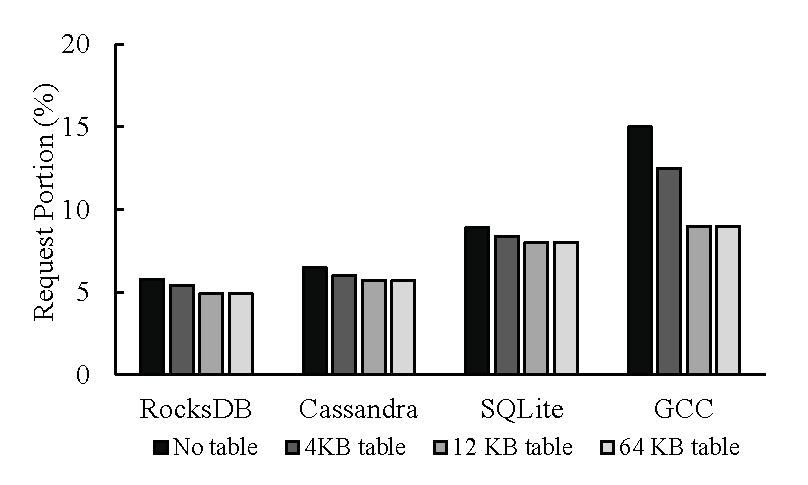
\includegraphics[width=0.7\linewidth]{figure/pctable}
	%\caption{The effect of the PC attribute table on the default stream allocation.}
	\caption{\note{The effect of the PC attribute table.}}
	\label{fig:pctable}
	\vspace{-10pt}
\end{figure}


We have presented a new stream management technique, \textsf{\small PCStream},
for multi-streamed SSDs.  Unlike existing techniques, \textsf{\small PCStream}
fully automates the process of mapping data to a stream based on PCs.  Based on
observations that most PCs are effective to distinguish lifetime
characteristics of written data, \textsf{\small PCStream} allocates each PC to
a different stream.  When a PC has a large variance in their lifetimes,
\textsf{\small PCStream} refines its stream allocation during GC and moves the
long-lived data of the current stream to the corresponding internal stream.
Our experimental results show that \textsf{\small PCStream} can improve the
IOPS by up to 56\% over the existing automatic technique while reducing WAF by
up to 69\%. 

The current version of \textsf{\small PCStream} can be extended in several
directions.  First, \textsf{\small PCStream} does not support applications that
rely on a write buffer ({\it e.g.,} MySQL). To address this, we plan to extend
\textsf{\small PCStream} interfaces so that developers can easily incorporate
\textsf{\small PCStream} into their write buffering modules with minimal
efforts.  Second, we have only considered write-related systems calls to
collect PCs, but many applications ({\it e.g.,} MonetDB~\cite{MonetDB}) heavily
access files with mmap-related functions ({\it e.g.}, \texttt{mmap()} and
\texttt{msync()}).  We plan to extend \textsf{\small PCStream} to work with
mmap-intensive applications. 

